\renewcommand{\theequation}{\theenumi}
\begin{enumerate}[label=\thesection.\arabic*.,ref=\thesection.\theenumi]
\numberwithin{equation}{enumi}

\item 
Given,
\begin{align}
    12x^2+7xy-10y^2+13x+45y-35&=0 
\label{eq:pair_given}
\end{align}

it is easy to verify that
\begin{align}
\mydet{
12 &\frac{7}{2}& \frac{13}{2}
\\
\frac{7}{2} & -10 & \frac{45}{2}
\\ 
\frac{13}{2} & \frac{45}{2} & -35
} = 0
\end{align}
%
Hence, \eqref{eq:pair_given} represents a pair of straight lines.
%
 \eqref{eq:pair_given} can be expressed as \eqref{eq:conic_quad_form} with
\begin{align}
    \vec{V}=\vec{V}^T&=\myvec{12 & \frac{7}{2}\\\frac{7}{2} &-10}\label{eq:pair_v}\\
    \vec{u}&=\myvec{\frac{13}{2} \\ \frac{45}{2}}\label{eq:pair_u}\\
    f&=-35\label{eq:pair_fv}
\end{align}
From \eqref{eq:pair_given} and \eqref{eq:quad_pair_slopes},
\begin{align}
\label{eq:quad_pair_slopes_ex}
\implies m_i &= \frac{-7 \pm \sqrt{49+480}}{-20}
\\
\implies m_1 &=  \frac{3}{2}, m_2 = -\frac{4}{5}
\end{align}
Thus,
\begin{align}
\vec{m}_1 = \myvec{2\\3},
\vec{m}_2 = \myvec{5\\-4}
\\
\implies
\vec{n}_1 = \myvec{3\\-2},
\vec{n}_2 = \myvec{4\\5}
\label{eq:quad_pair_norm_vec}
\end{align}
 Using the Toeplitz matrix,
\begin{align}
\vec{n}_1*\vec{n}_2 = 
\myvec{3 & 0
\\
-2 & 3
\\
0 & -2
}
\myvec{4\\5}
= \myvec{12 \\ 7 \\ -10}
\end{align}
%
which matches the corresponding coefficients in \eqref{eq:pair_given}

 Substituting from \eqref{eq:quad_pair_norm_vec}
in 
%\eqref{eq:quad_pair_ci_mat}, 
the augmented matrix is
\begin{align}
\myvec{
3 & 4 & -13
\\
-2 & 5 & -45
}
\xleftrightarrow[R_1 \leftarrow \frac{R_1 - 4R_2}{3}]{R_2 \leftarrow \frac{2R_1 + 3R_2}{23}}
\myvec{
1 & 0 & 5
\\
0 & 1 & -7
}
\\
\implies c_1 = -7, c_2 = 5
\end{align}

Fig.     \ref{fig:pair} plots the lines in \eqref{eq:pair_given}
%
\begin{figure}[h]
    \centering
    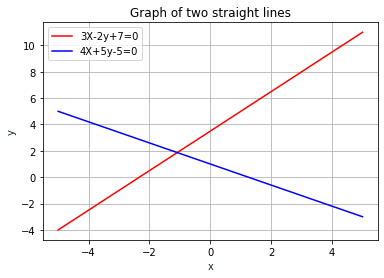
\includegraphics[width=\columnwidth]{./figs/pair/pair_ang.png}
    \caption{Pair of straight lines}
    \label{fig:pair}
\end{figure}

 From \eqref{eq:quad_pair_norm_vec}
the angle between the two straight lines is given by 
\begin{align}
    \theta&=\cos^{-1}\brak{\frac{\vec{n_1}^T\vec{n_2}}{\norm{\vec{n_1}}\norm{\vec{n_2}}}}
%\label{eq:pair_t}
\label{eq:pair_theta}
\\
    \vec{n_1}^T\vec{n_2}&=\myvec{3 & -2}\myvec{4\\5}=2\label{eq:pair_tr}\\
    \norm{\vec{n_1}}&=\sqrt{3^2+(-2)^2}=\sqrt{13}\label{eq:pair_norm1}\\
    \norm{\vec{n_2}}&=\sqrt{4^2+5^2}=\sqrt{41}\label{eq:pair_norm2}
\end{align}
Substituting equations \eqref{eq:pair_tr}, \eqref{eq:pair_norm1} ,\eqref{eq:pair_norm2} in equation \eqref{eq:pair_theta}, we get 
\begin{align}
        \theta&=\cos^{-1}\biggl(\frac{2}{\sqrt{13}\sqrt{41}}\biggr)\\
        \theta&=85\degree
\end{align}


\end{enumerate}

